\chapter{The Extrinsic Semiconductor}
\label{ch:extrinsic-semiconductor}

Sze and Lee introduce extrinsic semiconductors through substitutional donors
and acceptors, impurity levels, complete ionization, compensation, and the three
temperature regimes of freeze-out, extrinsic behavior, and intrinsic behavior
\cite[Sec.~1.6]{szeLee2012}.  This chapter retains that device-oriented
sequence while making the statistical closure explicit.  The localized-state
degeneracy factors and exact charge-neutrality problem are compared with Sze
and Ng \cite[Secs.~1.4.2--1.4.3]{szeNg2007}, and Rudan's treatment is used to
connect the dopant states to the periodic crystal, full Fermi integrals,
nonuniform electrostatics, compensation, and band-gap narrowing
\cite[Secs.~18.4--18.6]{rudan2015}.

\section{What doping changes---and what it does not}

\begin{definition}{Extrinsic semiconductor}{extrinsic-semiconductor}
An extrinsic semiconductor is a semiconductor whose equilibrium carrier
populations are intentionally modified by electrically active impurities or
defects.  Donors tend to provide conduction-band electrons; acceptors tend to
provide valence-band holes.  The actual populations are determined by the
band structure, dopant charge states, temperature, chemical potential, and
charge neutrality.
\end{definition}

Doping does not simply append a prescribed number of mobile particles.  A
concentration $N_D$ of donor atoms is not automatically the same as a
concentration $n=N_D$ of conduction electrons.  The equality requires at least
complete donor ionization, negligible compensation, and a regime in which
intrinsic carriers do not dominate.  Similarly, $p=N_A$ is a limiting result
for acceptors, not the definition of an acceptor.

Dilute substitutional impurities also do not erase the host bands.  To first
approximation, the periodic host still supplies its conduction and valence
bands, while each dilute impurity supplies a localized state in or near the
gap.  At high impurity concentrations this separation fails: localized states
overlap, impurity bands form, the band edges change, and many-body corrections
become important.

\section{Substitutional donors and acceptors}

In group-IV silicon, a substitutional group-V atom such as phosphorus has five
valence electrons.  Four participate in covalent bonds with neighboring
silicon atoms; the fifth is weakly bound.  Removing that electron to the
conduction band leaves a fixed positive donor ion:
\begin{equation}
  D^0\longrightarrow D^+ + e^-_{\mathrm C}.
  \label{eq:donor-ionization-reaction}
\end{equation}
A group-III atom such as boron has only three valence electrons.  It can accept
an electron from the valence band, leaving one mobile hole and one fixed
negative acceptor ion:
\begin{equation}
  A^0\longrightarrow A^- + h^+_{\mathrm V}.
  \label{eq:acceptor-ionization-reaction}
\end{equation}
Common group-V donors in silicon include phosphorus, arsenic, and antimony;
common group-III acceptors include boron, aluminum, gallium, and indium
\cite[Sec.~1.6.1]{szeLee2012}.  The mobile carriers belong to extended band
states.  The ionized dopant charges remain attached to lattice sites and
contribute to electrostatics, not to band transport as mobile particles.

\begin{figure}[H]
  \centering
  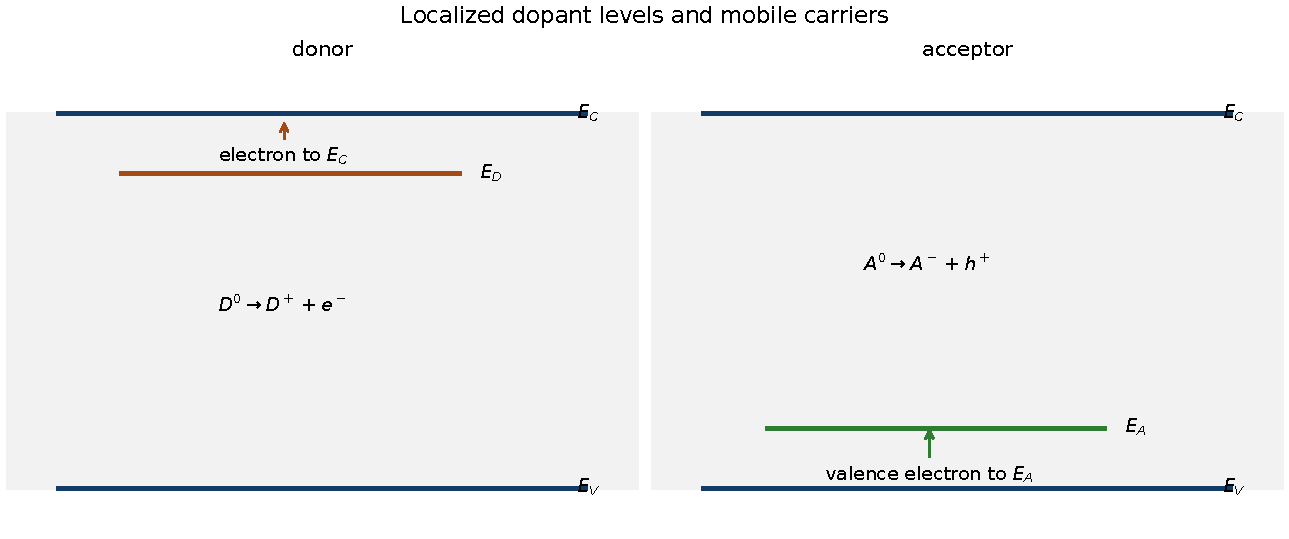
\includegraphics[width=0.88\textwidth]
    {figures/extrinsic-dopant-levels.pdf}
  \caption{Schematic donor and acceptor ionization.  A shallow donor level lies
  below $\Ec$ by the donor binding energy; a shallow acceptor level lies above
  $\Ev$ by the acceptor binding energy.  The drawing is not to scale.\figurenotebookmark}
  \label{fig:extrinsic-dopant-levels}
\end{figure}
\figurenotebooktext{figures/07_extrinsic-semiconductor/fig_07_01.ipynb}

\begin{table}[H]
  \centering
  \caption{Charge-state bookkeeping for singly ionizable dopants.}
  \label{tab:dopant-charge-states}
  \begin{tabularx}{\textwidth}{@{}
    >{\raggedright\arraybackslash}p{0.18\textwidth}
    >{\raggedright\arraybackslash}p{0.19\textwidth}
    >{\raggedright\arraybackslash}p{0.25\textwidth}
    >{\raggedright\arraybackslash}X@{}}
    \toprule
    Species & State & Localized electronic occupancy & Charge relative to host \\
    \midrule
    Donor & $D^0$ & donor electron bound & neutral \\
    Donor & $D^+$ & donor state empty & $+q$ \\
    Acceptor & $A^0$ & acceptor state empty & neutral \\
    Acceptor & $A^-$ & acceptor state filled by an electron & $-q$ \\
    \bottomrule
  \end{tabularx}
\end{table}

The notation prevents a common sign mistake: an ionized donor is positive
because it has lost an electron, while an ionized acceptor is negative because
it has gained one.

\section{Why shallow dopants resemble hydrogen}

A shallow donor electron is weakly bound and extends over many unit cells.  In
the simplest effective-mass model, the rapidly varying lattice-scale part has
already been absorbed into the band effective mass, and the remaining envelope
obeys a screened hydrogenic equation:
\begin{equation}
  \left[
    -\frac{\hbar^2}{2m_c^*}\nabla^2
    -\frac{q^2}{4\pi\varepsilon_s r}
  \right]F(\bm r)
  =-E_{B,D}F(\bm r).
  \label{eq:effective-mass-donor-hamiltonian}
\end{equation}
Relative to vacuum hydrogen, two replacements have occurred:
\begin{equation}
  m_0\longrightarrow m_c^*,
  \qquad
  \varepsilon_0\longrightarrow\varepsilon_s.
  \label{eq:hydrogenic-donor-replacements}
\end{equation}
The ground-state binding energy is therefore
\begin{equation}
\begin{aligned}
  E_{B,D}
  &=\frac{m_c^*q^4}
    {2(4\pi\varepsilon_s)^2\hbar^2}\\
  &=\left(\frac{m_c^*}{m_0}\right)
    \left(\frac{\varepsilon_0}{\varepsilon_s}\right)^2
    \SI{13.6}{\electronvolt}.
\end{aligned}
  \label{eq:effective-donor-binding-energy}
\end{equation}
The donor energy level is
\begin{equation}
  E_D=\Ec-E_{B,D}.
  \label{eq:donor-level-from-binding-energy}
\end{equation}
The effective Bohr radius is
\begin{equation}
\begin{aligned}
  a_D^*
  &=\frac{4\pi\varepsilon_s\hbar^2}{m_c^*q^2}\\
  &=\left(\frac{\varepsilon_s}{\varepsilon_0}\right)
    \left(\frac{m_0}{m_c^*}\right)a_0.
\end{aligned}
  \label{eq:effective-donor-bohr-radius}
\end{equation}
A large dielectric constant weakens the Coulomb attraction, and a small
effective mass raises the kinetic cost of localization.  Both effects reduce
the binding energy and enlarge the orbital, explaining why shallow-donor wave
functions can cover many lattice sites.

The analogous acceptor model replaces the conduction electron mass by an
appropriate hole mass and gives
\begin{equation}
  E_A=\Ev+E_{B,A}.
  \label{eq:acceptor-level-from-binding-energy}
\end{equation}
Within this scale estimate, Sze and Lee quote donor ionization energies of about
\SI{0.025}{\electronvolt} in silicon and \SI{0.007}{\electronvolt} in gallium
arsenide, and an acceptor scale of about \SI{0.05}{\electronvolt} in both
materials \cite[Sec.~1.6.1]{szeLee2012}.  These are pedagogical hydrogenic
estimates rather than universal species-resolved measurements.  The
\SI{45}{\milli\electronvolt} value used later in the illustrative silicon
calculation is a representative shallow-donor binding scale, deliberately
showing that a computational model must declare its chosen dopant parameter.

\begin{boundarybox}
The hydrogenic model predicts the correct scale for many shallow impurities,
but it is not a universal impurity theory.  Anisotropic and multivalley bands,
valence-band mixing, central-cell corrections, chemical bonding, multiple
charge states, and deep defects require more detailed models.  A deep level
should not be forced into a shallow-dopant formula merely because both appear
inside the gap.
\end{boundarybox}

\section{Localized-state statistics and degeneracy}

Band states form a continuum and use the Fermi--Dirac occupation derived from
the grand partition function in \cref{ch:statistical-mechanics-carriers}.  A
dilute donor or acceptor level is a
localized state with a small number of charge configurations.  Its occupation
therefore includes the degeneracies of those configurations.

This chapter adopts the Sze--Ng convention
\cite[Sec.~1.4.3]{szeNg2007}:
\begin{equation}
  \boxed{
  N_D^+
  =\frac{N_D}
   {1+g_D\exp[(\mu-E_D)/(\kb T)]},
  \qquad g_D=2,
  }
  \label{eq:ionized-donor-concentration}
\end{equation}
and
\begin{equation}
  \boxed{
  N_A^-
  =\frac{N_A}
   {1+g_A\exp[(E_A-\mu)/(\kb T)]},
  \qquad g_A=4.
  }
  \label{eq:ionized-acceptor-concentration}
\end{equation}
The numerical degeneracy factor is inseparable from the convention used to
place it in the formula.  Rudan, for example, parameterizes the localized-state
probabilities with an inverse degeneracy coefficient
\cite[Secs.~18.4.1--18.4.2]{rudan2015}.  Copying a bare value such as 2 or 4
between conventions without copying its defining equation gives the wrong
ionized fraction.

\subsection{Donor partition argument}

A singly ionizable donor has two relevant configurations: the empty, positively
charged state $D^+$ and the occupied, neutral state $D^0$.  Let the statistical
weight of $D^+$ define the reference.  The occupied state has the relative grand
canonical weight
\begin{equation}
  \frac{w(D^0)}{w(D^+)}
  =g_D\exp\left(\frac{\mu-E_D}{\kb T}\right).
  \label{eq:donor-relative-statistical-weight}
\end{equation}
Normalizing the two weights gives
\begin{equation}
\begin{aligned}
  \mathbb P(D^+)
  &=\frac{w(D^+)}{w(D^+)+w(D^0)}\\
  &=\frac{1}
   {1+g_D\exp[(\mu-E_D)/(\kb T)]},
\end{aligned}
  \label{eq:donor-ionization-probability-derivation}
\end{equation}
which yields \cref{eq:ionized-donor-concentration} after multiplication by
$N_D$.  Raising $\mu$ makes electron occupation more favorable and therefore
reduces the positive ionized fraction.

\subsection{Acceptor partition argument}

For an acceptor, the negatively charged state $A^-$ contains the captured
electron.  Under the adopted convention, the ratio of neutral to ionized
weights is
\begin{equation}
  \frac{w(A^0)}{w(A^-)}
  =g_A\exp\left(\frac{E_A-\mu}{\kb T}\right).
  \label{eq:acceptor-relative-statistical-weight}
\end{equation}
Therefore
\begin{equation}
\begin{aligned}
  \mathbb P(A^-)
  &=\frac{w(A^-)}{w(A^-)+w(A^0)}\\
  &=\frac{1}
   {1+g_A\exp[(E_A-\mu)/(\kb T)]},
\end{aligned}
  \label{eq:acceptor-ionization-probability-derivation}
\end{equation}
which gives \cref{eq:ionized-acceptor-concentration}.  Raising $\mu$ now makes
capture of an electron more favorable and increases the negative ionized
fraction.

\begin{figure}[H]
  \centering
  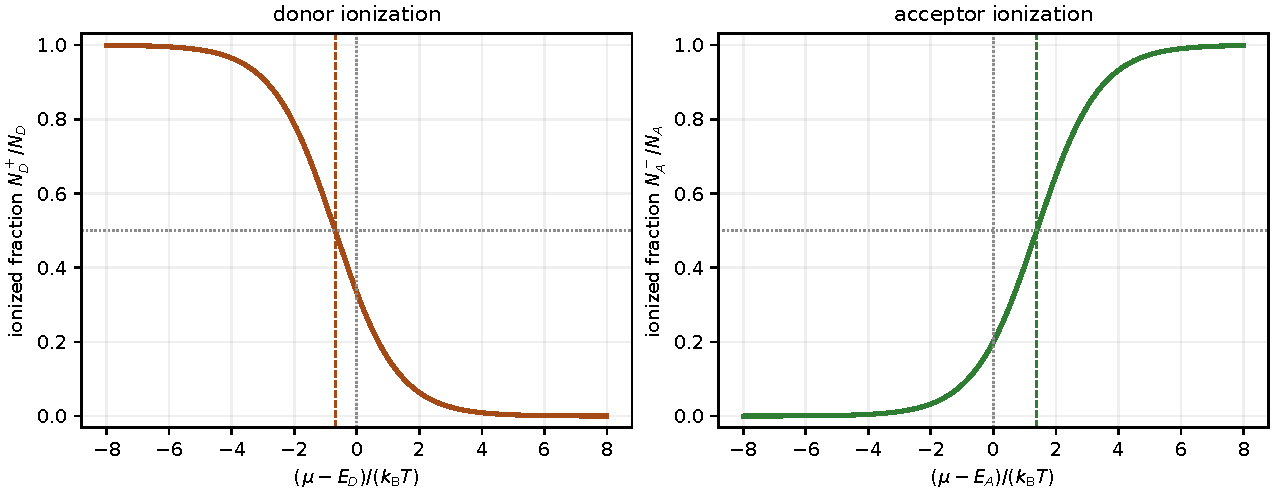
\includegraphics[width=0.88\textwidth]
    {figures/extrinsic-ionization-fractions.pdf}
  \caption{Ionized donor and acceptor fractions using the Sze--Ng degeneracy
  convention.  The half-ionization point is displaced from $\mu=E_D$ or
  $\mu=E_A$ by the logarithm of the corresponding degeneracy factor.\figurenotebookmark}
  \label{fig:extrinsic-ionization-fractions}
\end{figure}
\figurenotebooktext{figures/07_extrinsic-semiconductor/fig_07_02.ipynb}

Indeed, setting either fraction to one half gives
\begin{align}
  \mu_{D,1/2}&=E_D-\kb T\ln g_D,
  \label{eq:donor-half-ionization-level}\\
  \mu_{A,1/2}&=E_A+\kb T\ln g_A.
  \label{eq:acceptor-half-ionization-level}
\end{align}
This is why the statement ``a level is half occupied when $\mu$ equals the
level energy'' is not automatically valid for a degenerate localized state.

\section{The master charge-neutrality problem}

For a spatially uniform semiconductor containing both donors and acceptors, the
charge density is
\begin{equation}
  \rho
  =q\bigl[p+N_D^+-n-N_A^-\bigr].
  \label{eq:extrinsic-charge-density}
\end{equation}
Thermal equilibrium in a neutral bulk region requires
\begin{equation}
  \boxed{
  n+N_A^-=p+N_D^+.
  }
  \label{eq:extrinsic-charge-neutrality}
\end{equation}
This is the central closure equation of the extrinsic problem.  Every term is a
concentration of charge with a declared sign.  The equation does not say that
$n=N_D$ or $p=N_A$; those approximations may emerge after solving it.

With parabolic bands and full Fermi--Dirac statistics,
\begin{align}
  n(\mu,T)
  &=\Nc F_{1/2}\left(\frac{\mu-\Ec}{\kb T}\right),
  \label{eq:extrinsic-exact-electrons}\\
  p(\mu,T)
  &=\Nv F_{1/2}\left(\frac{\Ev-\mu}{\kb T}\right).
  \label{eq:extrinsic-exact-holes}
\end{align}
Substituting
\cref{eq:ionized-donor-concentration,eq:ionized-acceptor-concentration}
produces one nonlinear equation for $\mu$:
\begin{equation}
\begin{aligned}
  R(\mu)={}&
  \Nc F_{1/2}\left(\frac{\mu-\Ec}{\kb T}\right)
  +\frac{N_A}{1+g_Ae^{(E_A-\mu)/(\kb T)}}\\
  &-\Nv F_{1/2}\left(\frac{\Ev-\mu}{\kb T}\right)
  -\frac{N_D}{1+g_De^{(\mu-E_D)/(\kb T)}}=0.
\end{aligned}
  \label{eq:extrinsic-master-residual}
\end{equation}
As $\mu$ increases, $n$ and $N_A^-$ increase while $p$ and $N_D^+$ decrease.
Consequently $R(\mu)$ is monotonic under this model, making a bracketed scalar
root solver a natural numerical method.  The returned chemical potential is
acceptable only if the neutrality residual is small compared with the largest
charge concentration in the calculation.

\section{Nondegenerate carrier relations}

When the chemical potential lies several $\kb T$ from both band edges,
\begin{align}
  n&=\Nc\exp\left[-\frac{\Ec-\mu}{\kb T}\right],
  \label{eq:extrinsic-boltzmann-electrons}\\
  p&=\Nv\exp\left[-\frac{\mu-\Ev}{\kb T}\right].
  \label{eq:extrinsic-boltzmann-holes}
\end{align}
Using the intrinsic quantities derived in
\cref{ch:intrinsic-semiconductor}, these may be rewritten as
\begin{align}
  n&=n_i\exp\left(\frac{\mu-\mui}{\kb T}\right),
  \label{eq:electron-concentration-relative-intrinsic}\\
  p&=n_i\exp\left(-\frac{\mu-\mui}{\kb T}\right).
  \label{eq:hole-concentration-relative-intrinsic}
\end{align}
Multiplication gives the equilibrium mass-action law
\begin{equation}
  np=n_i^2.
  \label{eq:extrinsic-mass-action-law}
\end{equation}
A donor raises $\mu$, increasing $n$ exponentially while decreasing $p$ by the
same exponential factor.  An acceptor lowers $\mu$ and reverses those roles.
The dopant changes the balance between carrier types; it does not violate
thermal equilibrium.

\section{Complete ionization and compensation}

Suppose all shallow donors and acceptors are ionized:
\begin{equation}
  N_D^+\simeq N_D,
  \qquad
  N_A^-\simeq N_A.
  \label{eq:complete-ionization}
\end{equation}
Define the net doping
\begin{equation}
  \Delta N=N_D-N_A.
  \label{eq:net-doping}
\end{equation}
Charge neutrality becomes
\begin{equation}
  n-p=\Delta N.
  \label{eq:full-ionization-neutrality}
\end{equation}
Use $p=n_i^2/n$ to obtain
\begin{equation}
  n^2-\Delta N\,n-n_i^2=0.
  \label{eq:compensated-electron-quadratic}
\end{equation}
The physical positive root is
\begin{equation}
  \boxed{
  n=\frac{\Delta N+\sqrt{\Delta N^2+4n_i^2}}{2}.
  }
  \label{eq:compensated-electron-solution}
\end{equation}
Similarly,
\begin{equation}
  \boxed{
  p=\frac{-\Delta N+\sqrt{\Delta N^2+4n_i^2}}{2}.
  }
  \label{eq:compensated-hole-solution}
\end{equation}
These two equations cover n-type, intrinsic, compensated, and p-type limits
without changing formulas.

\begin{figure}[H]
  \centering
  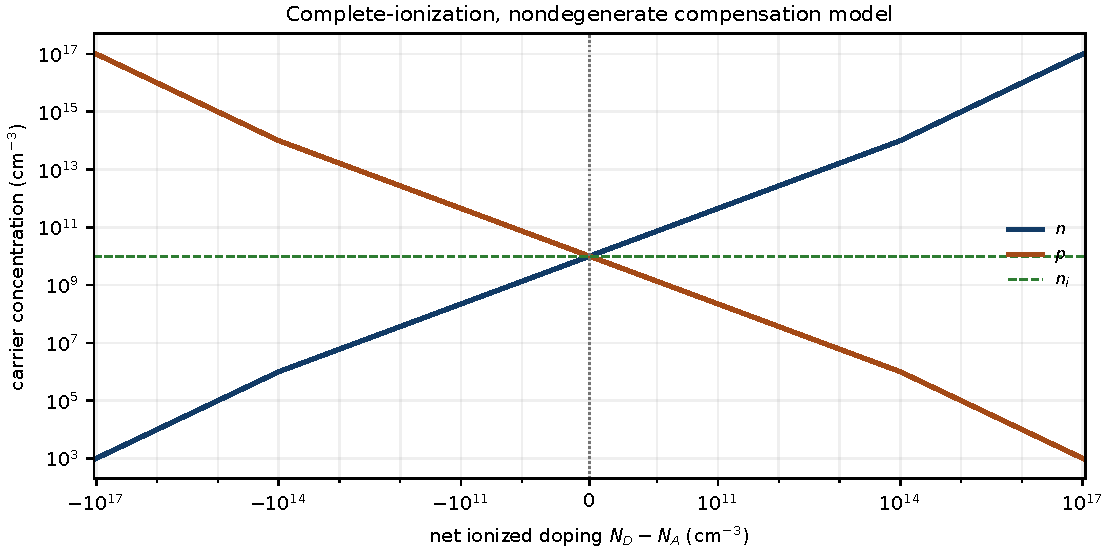
\includegraphics[width=0.82\textwidth]
    {figures/extrinsic-compensation.pdf}
  \caption{Carrier populations versus net ionized doping in the complete-
  ionization, nondegenerate model.  The transition through compensation is
  continuous; the majority-carrier approximation fails when
  $|N_D-N_A|$ is comparable to $n_i$.\figurenotebookmark}
  \label{fig:extrinsic-compensation}
\end{figure}
\figurenotebooktext{figures/07_extrinsic-semiconductor/fig_07_03.ipynb}

\subsection{Strong n-type limit}

If $\Delta N\gg n_i$, expand
\begin{equation}
  \sqrt{\Delta N^2+4n_i^2}
  =\Delta N
   \sqrt{1+\frac{4n_i^2}{\Delta N^2}}
  \simeq\Delta N+\frac{2n_i^2}{\Delta N}.
  \label{eq:n-type-square-root-expansion}
\end{equation}
Equations~\eqref{eq:compensated-electron-solution} and
\eqref{eq:compensated-hole-solution} reduce to
\begin{equation}
  n\simeq\Delta N,
  \qquad
  p\simeq\frac{n_i^2}{\Delta N}.
  \label{eq:n-type-majority-minority-limit}
\end{equation}
Electrons are majority carriers and holes are minority carriers.  The minority
population is small but not identically zero.

\subsection{Strong p-type limit}

If $-\Delta N\gg n_i$,
\begin{equation}
  p\simeq-\Delta N=N_A-N_D,
  \qquad
  n\simeq\frac{n_i^2}{N_A-N_D}.
  \label{eq:p-type-majority-minority-limit}
\end{equation}
Holes are now majority carriers and electrons are minority carriers.

\subsection{Fully compensated material}

When $N_D=N_A$ under complete ionization, $\Delta N=0$ and
\begin{equation}
  n=p=n_i.
  \label{eq:full-compensation-intrinsic-populations}
\end{equation}
The crystal is not chemically intrinsic: it contains charged donors and
acceptors.  It is electrically compensated in this ideal bulk model.  The
impurities can still affect scattering, lifetime, disorder, and band edges even
though the mobile equilibrium concentrations equal their intrinsic values.

\section{Fermi level in the complete-ionization regime}

In a strongly n-type, nondegenerate semiconductor with negligible
compensation,
\begin{equation}
  n\simeq N_D.
  \label{eq:full-ionization-n-type-concentration}
\end{equation}
Substituting into the conduction-band carrier relation gives
\begin{equation}
  \boxed{
  \Ec-\mu
  =\kb T\ln\left(\frac{\Nc}{N_D}\right).
  }
  \label{eq:n-type-fermi-level-from-donors}
\end{equation}
Equivalently,
\begin{equation}
  \mu-\mui
  =\kb T\ln\left(\frac{N_D}{n_i}\right).
  \label{eq:n-type-fermi-level-intrinsic-reference}
\end{equation}
Increasing $N_D$ moves $\mu$ upward toward $\Ec$.  For p-type material,
\begin{equation}
  \boxed{
  \mu-\Ev
  =\kb T\ln\left(\frac{\Nv}{N_A}\right),
  }
  \label{eq:p-type-fermi-level-from-acceptors}
\end{equation}
and
\begin{equation}
  \mui-\mu
  =\kb T\ln\left(\frac{N_A}{n_i}\right).
  \label{eq:p-type-fermi-level-intrinsic-reference}
\end{equation}
Increasing $N_A$ moves $\mu$ downward toward $\Ev$.

These logarithmic equations contain their own warning.  If a trial doping makes
$\mu$ approach a band edge within a few $\kb T$, the Boltzmann approximation
used to derive them is failing, and the full Fermi integral must replace it.

\section{Incomplete ionization and freeze-out}

At sufficiently low temperature, many dopant-bound carriers lack the thermal
energy required to reach the relevant band.  Consider uncompensated donor
doping, neglect holes, and retain nondegenerate band statistics.  Neutrality is
\begin{equation}
  n=N_D^+.
  \label{eq:freezeout-donor-neutrality}
\end{equation}
The band electron concentration gives
\begin{equation}
  e^{(\mu-\Ec)/(\kb T)}=\frac{n}{\Nc}.
  \label{eq:freezeout-eliminate-mu-1}
\end{equation}
Let the donor ionization energy be
\begin{equation}
  E_{I,D}=\Ec-E_D>0.
  \label{eq:donor-ionization-energy}
\end{equation}
Then
\begin{equation}
\begin{aligned}
  e^{(\mu-E_D)/(\kb T)}
  &=e^{(\mu-\Ec)/(\kb T)}
    e^{(\Ec-E_D)/(\kb T)}\\
  &=\frac{n}{\Nc}e^{E_{I,D}/(\kb T)}.
\end{aligned}
  \label{eq:freezeout-eliminate-mu-2}
\end{equation}
Substitution into the donor-ionization formula and use of $n=N_D^+$ gives
\begin{equation}
  \frac{g_D}{\Nc}e^{E_{I,D}/(\kb T)}n^2+n-N_D=0.
  \label{eq:donor-freezeout-quadratic}
\end{equation}
The positive solution is
\begin{equation}
  n
  =\frac{\Nc e^{-E_{I,D}/(\kb T)}}{2g_D}
   \left[
     \sqrt{1+\frac{4g_DN_D}{\Nc}
       e^{E_{I,D}/(\kb T)}}-1
   \right].
  \label{eq:donor-freezeout-exact-quadratic-solution}
\end{equation}
Deep in freeze-out, the quadratic term dominates the linear term in
\cref{eq:donor-freezeout-quadratic}, producing
\begin{equation}
  \boxed{
  n\simeq
  \sqrt{\frac{N_D\Nc}{g_D}}
  \exp\left(-\frac{E_{I,D}}{2\kb T}\right).
  }
  \label{eq:donor-freezeout-asymptote}
\end{equation}
The activation energy in this ideal uncompensated asymptote is one half of the
donor binding energy because the chemical potential moves as ionization
proceeds.  Reading a freeze-out slope as $E_{I,D}$ without deriving the relevant
limit can therefore introduce a factor-of-two error.

For uncompensated acceptors, define
\begin{equation}
  E_{I,A}=E_A-\Ev>0.
  \label{eq:acceptor-ionization-energy}
\end{equation}
The same calculation yields
\begin{equation}
  p\simeq
  \sqrt{\frac{N_A\Nv}{g_A}}
  \exp\left(-\frac{E_{I,A}}{2\kb T}\right)
  \label{eq:acceptor-freezeout-asymptote}
\end{equation}
under the same idealized assumptions.  Compensation can change both the
prefactor and the observed activation behavior.

\section{Three temperature regimes}

The temperature dependence of a shallow-donor sample is commonly divided into
three regimes:
\begin{enumerate}
  \item \textbf{Freeze-out:} $N_D^+<N_D$ and the carrier concentration is
        controlled by dopant ionization.
  \item \textbf{Extrinsic or saturation regime:} the dopants are nearly fully
        ionized, intrinsic generation is still small, and
        $n\simeq N_D-N_A$ for net n-type material.
  \item \textbf{Intrinsic regime:} thermally generated electron--hole pairs
        outnumber the net dopant contribution, so $n\simeq p\simeq n_i$ and
        $\mu$ approaches $\mui$.
\end{enumerate}
The boundaries are crossovers rather than phase transitions.  Their locations
depend on the dopant energy, concentration, compensation, host gap, effective
densities of states, and the selected accuracy threshold.

\begin{figure}[H]
  \centering
  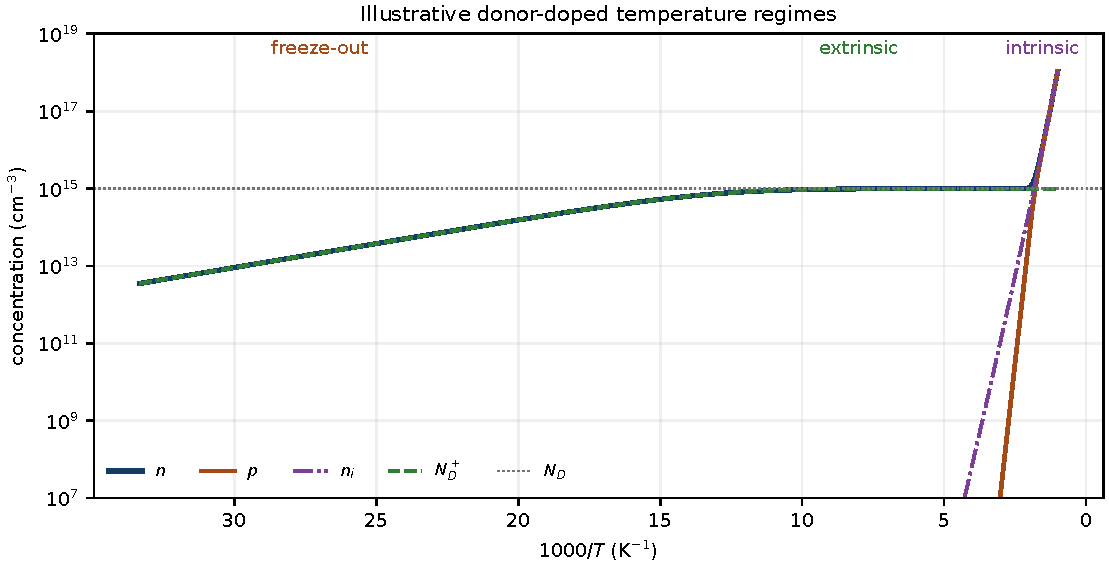
\includegraphics[width=0.84\textwidth]
    {figures/extrinsic-temperature-regimes.pdf}
  \caption{Illustrative donor-doped silicon calculation obtained by solving
  charge neutrality with partial donor ionization at every temperature.  The
  model uses $N_D=\SI{1e15}{\per\cubic\centi\metre}$,
  $E_{I,D}=\SI{45}{\milli\electronvolt}$, $g_D=2$, parabolic nondegenerate
  bands, and the same silicon gap and DOS convention used in
  \cref{ch:intrinsic-semiconductor}.  The curves are model evidence, not a
  substitute for a material-specific dopant dataset.\figurenotebookmark}
  \label{fig:extrinsic-temperature-regimes}
\end{figure}
\figurenotebooktext{figures/07_extrinsic-semiconductor/fig_07_04.ipynb}

The plot is often presented against $1/T$ because activated regimes become
approximately linear on a logarithmic vertical scale.  Care is still required:
$\Nc\propto T^{3/2}$, $\Eg$ varies with temperature, and $\mu$ is itself a
solution of neutrality, so no entire curve is described by one activation
energy.

\section{Worked n-type silicon estimate at \SI{300}{\kelvin}}

Following the illustrative Sze--Lee calculation
\cite[Example~4 in Sec.~1.6.1]{szeLee2012}, take
\begin{equation}
  N_D=\SI{1e16}{\per\cubic\centi\metre},
  \qquad
  N_A=0,
  \label{eq:worked-n-type-doping}
\end{equation}
with complete ionization and the convention
\begin{equation}
  n_i=\SI{9.65e9}{\per\cubic\centi\metre},
  \qquad
  \Nc=\SI{2.86e19}{\per\cubic\centi\metre},
  \qquad
  \kb T=\SI{0.0259}{\electronvolt}.
  \label{eq:worked-n-type-parameters}
\end{equation}
Because $N_D\gg n_i$,
\begin{equation}
  n\simeq N_D
  =\SI{1e16}{\per\cubic\centi\metre}.
  \label{eq:worked-n-type-electrons}
\end{equation}
The minority holes follow from mass action:
\begin{equation}
\begin{aligned}
  p
  &=\frac{n_i^2}{n}\\
  &=\frac{(9.65\times10^9)^2}{10^{16}}\\
  &\simeq\SI{9.3e3}{\per\cubic\centi\metre}.
\end{aligned}
  \label{eq:worked-n-type-holes}
\end{equation}
The distance from the conduction-band edge is
\begin{equation}
\begin{aligned}
  \Ec-\mu
  &=\kb T\ln\left(\frac{\Nc}{N_D}\right)\\
  &=0.0259\ln\left(\frac{2.86\times10^{19}}{10^{16}}\right)\\
  &\simeq\SI{0.205}{\electronvolt}.
\end{aligned}
  \label{eq:worked-n-type-fermi-edge-distance}
\end{equation}
The chemical potential is therefore still inside the gap and more than several
$\kb T$ below $\Ec$, so the nondegenerate approximation is self-consistent.
Using $\mui$ as the reference gives
\begin{equation}
  \mu-\mui
  =\kb T\ln\left(\frac{N_D}{n_i}\right)
  \simeq\SI{0.358}{\electronvolt}.
  \label{eq:worked-n-type-intrinsic-level-shift}
\end{equation}

\section{Degenerate doping and impurity-band limits}

When $\mu$ approaches or enters a band, the Boltzmann relations and the simple
mass-action law must be abandoned.  The full Fermi integrals in
\cref{eq:extrinsic-exact-electrons,eq:extrinsic-exact-holes} are then required.
High doping can also produce effects that are separate from degeneracy:
\begin{itemize}
  \item dopant wave functions overlap and broaden discrete impurity levels into
        impurity bands;
  \item ionized-impurity and carrier--carrier interactions modify the band
        edges;
  \item the effective gap can narrow;
  \item screening changes dopant binding energies; and
  \item simple independent localized-state occupations cease to be adequate.
\end{itemize}
Sze and Lee emphasize degeneracy and band-gap narrowing at high doping
\cite[Sec.~1.6.2]{szeLee2012}; Rudan treats impurity-band overlap and the
resulting effective band-edge shifts explicitly
\cite[Sec.~18.6]{rudan2015}.

If a model represents band-gap narrowing by shifts
$\Delta\Ec>0$ and $\Delta\Ev>0$,
\begin{equation}
  \Ec'=\Ec-\Delta\Ec,
  \qquad
  \Ev'=\Ev+\Delta\Ev,
  \label{eq:band-gap-narrowing-edge-shifts}
\end{equation}
then
\begin{equation}
  \Eg'=\Eg-\Delta\Eg,
  \qquad
  \Delta\Eg=\Delta\Ec+\Delta\Ev.
  \label{eq:band-gap-narrowing}
\end{equation}
Because intrinsic-like products depend exponentially on the gap, even a modest
$\Delta\Eg$ can strongly affect minority concentrations.  The correction must
be based on a declared empirical or many-body model rather than inserted as an
unlabeled fitting constant.

\section{Why local neutrality fails for nonuniform doping}

Equation~\eqref{eq:extrinsic-charge-neutrality} is appropriate for a uniform
neutral bulk region.  If $N_D$ or $N_A$ varies with position, carriers diffuse.
The immobile ionized dopants do not follow them, so a local space charge and an
electric field develop.  The general charge density is
\begin{equation}
  \rho(\bm r)
  =q\left[
    p(\bm r)-n(\bm r)
    +N_D^+(\bm r)-N_A^-(\bm r)
  \right],
  \label{eq:nonuniform-semiconductor-charge-density}
\end{equation}
and the electrostatic potential satisfies
\begin{equation}
  -\nabla\cdot\bigl(\varepsilon_s\nabla\phi\bigr)
  =\rho(\phi,\bm r).
  \label{eq:semiconductor-poisson-equation}
\end{equation}
Carrier and dopant occupations depend on the shifted local energies, so
\cref{eq:semiconductor-poisson-equation} is nonlinear and must be solved
self-consistently.  Replacing it pointwise by $\rho=0$ would erase depletion
regions, built-in fields, and junction electrostatics.

\section{Computational laboratory: solving neutrality}

The following compact calculation uses nondegenerate bands but retains partial
donor and acceptor ionization.  It brackets the chemical potential and verifies
the returned charge residual.  Energy quantities are in electronvolts and
concentrations are in \si{\per\cubic\centi\metre}.

\begin{lstlisting}[
  caption={Bracketed equilibrium solve with incomplete ionization.},
  label={lst:extrinsic-neutrality-solve}
]
from math import exp

KB_EV = 8.617333262145e-5
T = 300.0
EV = 0.0
EC = 1.12
ED = EC - 0.045
EA = EV + 0.045
NC = 2.86e19
NV = 2.66e19
ND = 1.0e16
NA = 2.0e15
GD = 2.0
GA = 4.0
thermal = KB_EV * T


def populations(mu):
    n = NC * exp((mu - EC) / thermal)
    p = NV * exp((EV - mu) / thermal)
    donor_plus = ND / (1.0 + GD * exp((mu - ED) / thermal))
    acceptor_minus = NA / (1.0 + GA * exp((EA - mu) / thermal))
    return n, p, donor_plus, acceptor_minus


def residual(mu):
    n, p, donor_plus, acceptor_minus = populations(mu)
    return n + acceptor_minus - p - donor_plus


lower = EV - 0.5
upper = EC + 0.5
assert residual(lower) < 0.0 < residual(upper)

for _ in range(200):
    middle = 0.5 * (lower + upper)
    if residual(middle) > 0.0:
        upper = middle
    else:
        lower = middle

mu = 0.5 * (lower + upper)
n, p, donor_plus, acceptor_minus = populations(mu)
scale = max(n, p, donor_plus, acceptor_minus)
assert abs(residual(mu)) / scale < 1.0e-12
assert 0.0 <= donor_plus <= ND
assert 0.0 <= acceptor_minus <= NA
assert abs(n * p - NC * NV * exp(-(EC - EV) / thermal)) / (n * p) < 1.0e-12
\end{lstlisting}

The calculation returns
\begin{equation}
\begin{aligned}
  \mu-\Ev&=\SI{0.9084}{\electronvolt},\\
  n&=\SI{7.968e15}{\per\cubic\centi\metre},\\
  p&=\SI{1.461e4}{\per\cubic\centi\metre},\\
  N_D^+&=\SI{9.968e15}{\per\cubic\centi\metre},\\
  N_A^-&=\SI{2.000e15}{\per\cubic\centi\metre}.
\end{aligned}
  \label{eq:extrinsic-laboratory-output}
\end{equation}
The six-per-cubic-centimetre absolute residual remaining in double precision is
less than $10^{-15}$ of the dominant concentration.  The code does not assume
$n=N_D-N_A$.  If complete ionization and strong net n-type behavior are valid,
that result should emerge from the solution and can then be used as a checked
approximation.

\section{Verification checklist}

An extrinsic-semiconductor calculation should establish that
\begin{enumerate}
  \item every dopant species has a declared chemical identity, lattice role,
        energy level, concentration, and degeneracy convention;
  \item $0\le N_D^+\le N_D$ and $0\le N_A^-\le N_A$;
  \item the charge-neutrality residual is small compared with the dominant
        charge density;
  \item the solution approaches the intrinsic result as $N_D,N_A\to0$;
  \item the complete-ionization quadratic is recovered when the ionized
        fractions approach unity;
  \item the majority and minority limits satisfy $np=n_i^2$ only where the
        nondegenerate approximation is valid;
  \item freeze-out, extrinsic, and intrinsic regimes are identified from the
        solved populations rather than imposed labels;
  \item Fermi-integral and band-gap-narrowing corrections are activated before
        their simplified assumptions fail; and
  \item a nonuniform doping profile is coupled to Poisson's equation instead of
        being forced into local neutrality.
\end{enumerate}

\section{Chapter summary}

Doping adds localized charge states to the host semiconductor and shifts the
equilibrium chemical potential.  Donor and acceptor concentrations become
mobile-carrier concentrations only through ionization statistics and charge
neutrality.  In the complete-ionization, nondegenerate regime, the familiar
majority-carrier estimates $n\simeq N_D-N_A$ or
$p\simeq N_A-N_D$ follow from a quadratic solution together with
$np=n_i^2$.  At low temperature, incomplete ionization produces freeze-out; at
high temperature, intrinsic pair generation dominates; and at high doping,
degeneracy, impurity bands, screening, and band-gap narrowing require richer
models.  The master principle is unchanged: solve the charged populations
self-consistently, then justify every reduction used to simplify them.
